\documentclass{article}
\usepackage{amsmath}
\usepackage{graphicx}
\usepackage{psfrag}
\newcommand{\argmin}{\mathop{\mathrm{argmin}}}
\newcommand{\infl}{\eta}
\newcommand{\Ind}{\mathrm{I}}

\title{A (Partial) Documentation of RBF \& AdaBoost$_{Reg}$ Software Packages}
\author{Gunnar R\"atsch}
\date{\today}
\begin{document}
\maketitle

\section{Overview}
The RBF and AdaBoost$_{Reg}$ packages consists out of eight
classes:\footnote{Please read the licensing and (no) warranty terms in
  Appendix \ref{app:terms}.}
\begin{itemize}
\item The data storage classes: {\tt data, data\_w},
\item the abstract learner classes: {\tt learner, learner\_w},
\item an implementation of an RBF network {\tt rbf\_net\_w} and
\item some classes for ensemble learning: {\tt booster\_base, adabooster, adabooster\_regul}.
\end{itemize}
All classes are implemented in MATLAB and should work with MATLAB R11 and R12
on almost any platform. The class hierarchy can be found in Figure
\ref{fig:hier}.
\begin{figure}[h]
\begin{center}
\psfrag{data}{{\tt data}}
\psfrag{dataw}{{\tt data\_w}}
\psfrag{rbf}{{\tt rbf\_net\_w}}
\psfrag{adabooster}{{\tt adabooster}}
\psfrag{boosterbase}{{\tt booster\_base}}
\psfrag{abreg}{{\tt adabooster\_regul}}
\psfrag{learner}{{\tt learner}}
\psfrag{learnerw}{{\tt learner\_w}}
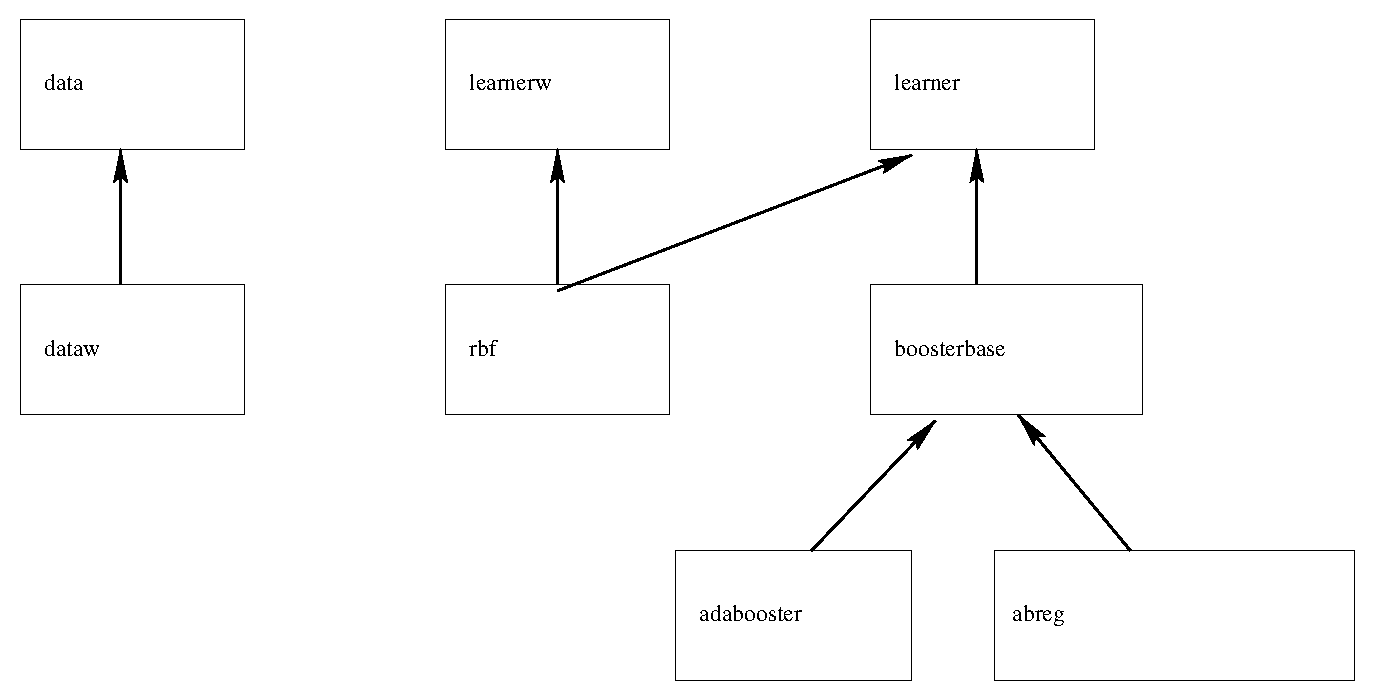
\includegraphics[width=\textwidth,height=4cm]{hier}
\end{center}
\caption{\label{fig:hier} Class-hierarchy of the classes in this package}
\end{figure}

\section{The data storage classes}

\subsection{Class {\tt data}: training, validation \& test set}

The class {\tt data} implements the basic functions for managing data sets
consisting of training, test and validation set. The methods of the class {\tt
  data} are:
\begin{itemize}
\item {\tt dataset=data(trainpat, traintarg, testpat, testtarg, valpat,
    valtarg);}\\
  This constructor creates a {\tt data} object with training set ({\tt
    trainpat, traintarg}), test set ({\tt testpat, testtarg}) and validation
  set ({\tt
    valpat, valtarg}).\\
  Example:
  \begin{verbatim}
    >> X=rand(1,200) ; Y=2*(X<0.3)-1 ;
    >> dataset=data(X(1,1:100), Y(1,1:100), ...
                    X(1,101:200), Y(1,101:200))
    data object
    the sname is : none
    the nsname is: none_tr100_v0_t100
      number of train patterns     : 100
      number of test patterns      : 100
      number of validation patterns: 0
      input dimension      : 1
      output dimension     : 1
    training data has not zero mean
    training data has not standard deviation one
  \end{verbatim}
\vspace*{-5mm}
\item {\tt [trainpat, traintarg]=get\_train(dataset, order);\\
    \ [testpat, testtarg]=get\_test(dataset,order);\\
    \ [valpat, valtarg]=get\_val(dataset,order)};\\
  These methods extract the data stored in the {\tt data} object. The first
  argument is the object created with the constructor above. If the parameter
  {\tt order} is not specified or {\tt order=1}, then the return arguments
  are {\tt [\{train,test,val\}pat, \{train,test,val\}targ]}. If {\tt order=2},
  the only {\tt [\{train,test,val\}targ]} is returned.
\item {\tt numpat=get\_train\_size(dataset);\\
    numpat=get\_test\_size(dataset);\\
    numpat=get\_val\_size(dataset)};\\
  Returns the number of samples of training, test or validation set for the
  given {\tt data} object.
\item {\tt odim=get\_odim(dataset);\\
    idim=get\_idim(dataset)}\\
  Returns the input or output dimension ({\tt odim} should be $1$) of the
  training, test and validation set (should be the same for all three sets).
\item {\tt dataset=split\_train(dataset, testsize, valsize);}\\
  Splits up the training set into training, test and validation set. {\tt
    testsize} and {\tt valsize} specify the size of the test and validation
  set after splitting. The rest is used as training data.
\item {\tt dataset=normalize(dataset) ;}\\
  Linearly transforms the data, such that the training set has zero-mean in
  all dimensions. The same transformation is applied to test and validation
  data.
\item {\tt dataset=standardize(dataset) ;}\\
  Linearly transforms the data, such that the training set has zero-mean and a
  standard deviation of $1$ in all dimensions. The same transformation is
  applied to test and validation data.
\end{itemize}

\subsection{Class {\tt data\_w}: weighted training data}
The class {\tt data\_w} extends the functionality of class {\tt data} to
allow weighted training sets as often used in Boosting/Ensemble learning
methods.  The methods of the class {\tt data\_w} are:
\begin{itemize}
\item {\tt dataset=data\_w(dataset)}\\
  This constructor creates a {\tt data\_w} object from an existing {\tt
    data} object.  \\
  Example:
  \begin{verbatim}
    >> X=rand(1,200) ; Y=2*(X<0.3)-1 ;
    >> dataset=data(X(1,1:100), Y(1,1:100), ...
                    X(1,101:200), Y(1,101:200)) ;
    >> datasetw=data_w(dataset) ;
  \end{verbatim}
\vspace*{-5mm}
\item {\tt datasetw=set\_sampl\_weights(datasetw, weights)\\
    weights=get\_sampl\_weights(datasetw)}\\
  Sets or gets the weights associated to the training set. The parameter {\tt
    weights} is a row-vector with length {\tt get\_train\_size(datasetw)}.
\end{itemize}

\section{Abstract Learner Classes}
\subsection{Class {\tt learner}}

The class {\tt learner} implements the abstract functionality of any
``learner''. The methods are:
\begin{itemize}
\item {\tt lrn=learner(idim, odim);}\\
  This constructor creates a {\tt learner} object for data of input dimension
  {\tt idim} and output dimension {\tt odim}. {\tt idim} and {\tt odim}
  default to $1$, if not given. 
\item {\tt lrn=do\_learn(lrn, dataset);}\\
  This is an abstract function which any derived class has to
  implement/overload. The learner {\tt lrn} is given a dataset and learns from
  the data. It may use the training and validation set only.
\item {\tt output\_data=calc\_output(lrn, in\_data);}\\
  This is an abstract function which any derived class has to
  implement/overload. After calling {\tt do\_learn}, one may use {\tt
    calc\_output} to compute the predictions of the learner based on the
  training/validation data.\\
  Example:
  \begin{verbatim}
    >> X=rand(2,200) ; Y=2*(X(1,:)+X(2,:)<0.7)-1 ;
    >> dataset=data(X(1,1:100), Y(1,1:100), ...
                    X(1,101:200), Y(1,101:200)) ;
    >> lrn= ... % some derived class from learner
    >> lrn=do_learn(lrn,dataset) ;
    >> output=calc_output(lrn, rand(1,200)) ;
  \end{verbatim}
  \vspace*{-5mm}
\item {\tt [trErrs, tstErrs, valErrs]=get\_class\_errors(lrn, dataset);}\\
  Computes the training, test and validation classification error rates if the
  learner is used for classification.
\item {\tt [trErrs, tstErrs, valErrs]=get\_mse(lrn, dataset);}\\
  Computes the training, test and validation mean squared error if the learner
  is used for regression.
\end{itemize}

\subsection{Class {\tt learner\_w}: Learning weighted data}
The class {\tt learner\_w} has the functionality needed for weighted training
sets. It is not derived from {\tt learner}. Any learner for weighted training
sets should be derived from {\tt learner} {\em and} {\tt learner\_w}. The
methods are:
\begin{itemize}
\item {\tt lrnw=learner\_w;}\\
Constructs the {\tt learner\_w} object.
\item {\tt weights=get\_distr(lrnw);\\
    lrnw=set\_distr(lrnw, weights);}\\
  Methods for setting and getting the distribution/weighting to the learner.
\item {\tt data\_w\_verify(lrnw, dataset)}\\
  Checks whether the given data set is a {\tt data\_w} object that eventually
  could be used for learning by an {\tt learner\_w} object.
\end{itemize}

\section{The RBF Network Class}
\subsection{Class {\tt rbf\_net\_w}}
The class {\tt rbf\_net\_w} implements the algorithm given in Appendix
\ref{app:rbf}. It has several methods for internal use only. The steps given
in the pseudo-code can be mapped to methods as follows: Initialization: {\tt
  cluster, private/clustknb\_new\_w}; 1. {\tt calc\_weights, private/update,
  private/ls\_solve\_w, private/design\_rbf}; 2a. {\tt private/rbfgrad\_w};
2b. {\tt private/optimize}; 3a. {\tt private/linmin, private/mnbrak,
  private/brent} and 3b. {\tt private/optimize}.

The class {\tt rbf\_net\_w} is derived from {\tt learner} and {\tt
  learner\_w}. The methods to be used are:
\begin{itemize}
\item {\tt lrn=rbf\_net\_w(numcen, lambda, idim, odim);}\\
  This constructor creates a {\tt rbf\_net\_w} object with {\tt numcen} centers
  and $\lambda=${\tt lambda}.
\item {\tt lrn=set\_max\_iter(lrn, maxiter);}\\
  Sets the maximum number of CG iterations (cf.~Figure~\ref{RBFALG}). This is
  the parameter which influences the learning speed most (default: 10).
\item {\tt lrn=do\_learn(lrn, dataset, do\_cluster);}\\
  This method overloads the abstract function defined in class {\tt learner}.
  The learner {\tt lrn} is given a dataset and learns from the given data. The
  parameter {\tt do\_cluster} is a boolean variable determining whether the
  centers should be initialized via K-means clustering (strongly recommended).
\item {\tt output\_data=calc\_output(lrn, in\_data);}\\
  This method overloads the abstract function defined in class {\tt learner}.
  After calling {\tt do\_learn}, one may use {\tt calc\_output} to compute the
  predictions of the learner based on the training/validation data.
\end{itemize}
Example:
\begin{verbatim}
    >> X=rand(2,200) ; Y=2*(X(1,:)+X(2,:)<0.7)-1 ;
    >> dataset=data(X(1,1:100), Y(1,1:100), ...
                    X(1,101:200), Y(1,101:200)) ;
    >> lrn=rbf_net_w(3, 1e-3, 2, 1) ; % 3 centers and lambda=0.001
    >> lrn=do_learn(lrn, dataset, 1) ;
    >> [trErr,teErr]=get_class_errors(lrn, dataset) 
    trErr =
        0.1500
    teErr =
        0.2300
\end{verbatim}

\section{The Ensemble Learning Classes}
\subsection{Class {\tt booster\_base}: the basis}
The class {\tt booster\_base} implements the basic functionality for all
ensemble learning classes. An object of this class stores a prototype (``base
learner'') of a learner object (base learner), an array of {\tt learner}
objects that are already trained (``base hypothesis'') and some additional
parameters like the number of iterations. The most important methods are:
\begin{itemize}
\item {\tt bb=booster\_base(prototype, boost\_steps, param1, param2);}\\
  Creates a {\tt booster\_base} object. The parameter {\tt prototype} is an
  object derived from {\tt learner} and optionally derived from {\tt
    learner\_w} (e.g.~{\tt rbf\_net\_w}). The parameter {\tt boost\_steps}
  determines the number of base hypothesis that should be combined. {\tt
    param1} and {\tt param2} are optional parameters that are given to the
  method {\tt do\_learn} of the base learner.
\item  {\tt wl=train\_weak(bb, dataset);}\\
  Calls {\bf do\_learn} of the prototype and returns the trained {\tt learner}
  object (base hypothesis).
\item {\tt weights=get\_vote\_weights(bb, idx);\\
    bb=set\_vote\_weights(bb, weights, idx);} \\
  Method for getting and setting the weights for linear combination of the
  base hypotheses.
\item {\tt lrn=get\_boosted\_learner(bb, idx);\\
    bb=set\_boosted\_learner(bb, lrn, idx);}\\
  Method for getting and setting the base hypothesis (objects of class {\tt
    learner}) for linear combination.
\end{itemize}

\subsection{Class {\tt adabooster}: the original AdaBoost algorithm}
The class {\tt adabooster} is derived from {\tt booster\_base} and implements
the original AdaBoost algorithm \cite{FreSch94} (cf.~pseudo-code in Figure
\ref{fig:ABALG}). It has several methods for internal use only. The steps given
in the pseudo-code can be mapped to methods as follows: Initialization: {\tt
  init\_learn}; 1. {\tt train\_week, do\_learn}; 2.\&3. {\tt comp\_weight,
  do\_learn} and 4. {\tt comp\_distr, do\_learn}. 
\begin{itemize}
\item {\tt bb=adabooster(proto, booststeps, param1, param2);}\\
  Constructor for {\tt adabooster} objects (cf.~{\tt booster\_base}).
\item {\tt bb=do\_learn(bb, dataset);}\\
  Implements the AdaBoost algorithm (cf.~Figure~\ref{fig:ABALG} and {\tt
    learner/do\_learn}).
\item {\tt weights=comp\_distr(bb, b\_t, output, dataset, weights, Prot,
    t);}\\
  Computes the new pattern distribution using the previous weights ({\tt
    weights}), the output of the previous base hypothesis ({\tt output}) and
  the weight of the last base hypothesis ({\tt b\_t}).
\item {\tt [bb, b\_t]=comp\_weight(bb, t, output, dataset, weights,
    EpsT);}\\
  Computes the weight {\tt b\_t} of the current base hypothesis based on its
  output ({\tt output}) on the training set, the previous pattern weights
  ({\tt weights}) and the weighted classification error ({\tt EpsT}).
\item {\tt Prot=report(bb, t, EpsT, weights, dataset, Prot);}\\
  This function is called in each iteration and can be used to make some
  outputs and/or to record some variables stored in the variable {\tt Prot}
  for later analysis.
\item  {\tt id=get\_use\_sign\_output(bb);\\
    bb=set\_use\_sign\_output(bb, id);}\\
  Sets or gets how the outputs of the base hypothesis are transformed: 0 - no
  transformation; 1 - signum function mapping to $\{-1,+1\}$ and 2 - sigmoidal
  transformation to [-1..+1].
\item {\tt bb=finish\_learn(bb);} \\
  Cleans up after learning.
\end{itemize}
Example:
\begin{verbatim}
    >> X=rand(2,200) ; Y=2*(X(1,:)+X(2,:)<0.7)-1 ;
    >> dataset=data(X(1,1:100), Y(1,1:100), ...
                    X(1,101:200), Y(1,101:200)) ;
    >> lrn=rbf_net_w(3, 1e-3, 2, 1) ; % 3 centers and lambda=0.001
    >> bb=adabooster(lrn, 30, 1) ; % 30 iterations
    >> bb=do_learn(bb,dataset) ;
    >> [trErr,teErr]=get_class_errors(bb, dataset) 
    trErr =
        0.1100
    teErr =
        0.2100
\end{verbatim}

\subsection{Class {\tt adabooster\_regul}: the regularized algorithm}
This class is derived from {\tt adabooster} and just adds/overloads some
functionality. The algorithm implemented in this class is given in
Figure~\ref{fig:ABREGALG} as pseudo-code.
\begin{itemize}
\item {\tt bb=adabooster\_regul(proto, booststeps, phi, C, param1, param2);}\\
  The constructor for this class. The parameter {\tt phi} modifies the error
  function (details are given in \cite{RaeOnoMue00a}, $\phi=\frac{1}{2}$ is a
  reasonable choice). The parameter C is the regularization parameter: $C=0$
  leads to the original AdaBoost algorithm. Large $C$ means a ``very soft
  margin''.
\end{itemize}
The other functions e.g.~{\tt do\_learn, comp\_distr} and {\tt comp\_weight} work
as before -- they just contain slightly different formulas.

\begin{appendix}
\section{Appendix}
\subsection{RBF nets with adaptive centers}
\label{app:rbf}

The RBF nets used in the experiments are an extension of the method of
\cite{MooDar89}, since centers and variances are also adapted (see also
\cite{Bis95,MueSmoRaeSchKohVap98}). The output of the network is
computed as a linear superposition of $K$ basis functions
\begin{equation}
  f({\bf x})=\sum_{k=1}^K w_k g_k({\bf x})~,
\end{equation}
where $w_k$, $k=1, \dots, K$, denotes the weights of the output layer.
The Gaussian basis functions $g_k$ are defined as
\begin{equation}
  g_k({\bf x})= \exp\left(-\frac{\|{\bf x}-{\bf \mu}_k\|^2}{2\,\sigma_k^2}\right),
\end{equation}
where ${\bf \mu}_k$ and $\sigma_k^2$ denote means and variances,
respectively. In a first step, the means ${\bf \mu}_k$ are initialized
with K-means clustering and the variances $\sigma_k$ are determined as
the distance between ${\bf \mu}_k$ and the closest ${\bf \mu}_i$
($i\ne k, i\in \{1,\ldots,K\}$). Then in the following steps we
perform a gradient descent in the regularized error function (weight
decay)
\begin{equation}
  E = \frac{1}{2}\sum_{i=1}^l \left(y_i - f({\bf x}_i)\right)^2 +
  \frac{\lambda}{2 l} \sum_{k=1}^K w_k^2.
\label{equ:rbf-reg} 
\end{equation}
%
%It is easy to derive the gradients $\partial E/\partial {\bf \mu}_k$
%and $\partial E/\partial \sigma_k$ (see later).  
%
Taking the derivative of (\ref{equ:rbf-reg}) with respect to
RBF means $\bf\mu_k$ and variances $\sigma_k$ we obtain
\begin{equation}
  \frac{\partial E}{\partial {\bf \mu}_k} =
    \sum_{i=1}^l (f({\bf x}_i)- y_i)\frac{\partial}{\partial {\bf \mu}_k}f({\bf x}_i), 
  \label{equ:grad_C_mu}
\end{equation}
with $\frac{\partial}{\partial {\bf \mu}_k} f({\bf x}_i) = w_k\frac{{\bf x}_i-{\bf
    \mu}_k}{\sigma_k^2} g_k({\bf x}_i)$ and
\begin{equation}
  \frac{\partial E}{\partial \sigma_k} = \sum_{i=1}^l
  \left(f({\bf x}_i)- y_i\right)
  \frac{\partial}{\partial \sigma_k} f({\bf x}_i), \label{equ:grad_C_sigma}
\end{equation}
with $\frac{\partial}{\partial \sigma_k}f({\bf x}_i) = w_k\frac{\|{\bf
    \mu}_k-{\bf x}_i\|^{2} }{\sigma_k^3} g_k({\bf x}_i)$.  These two derivatives are
employed in the minimization of (\ref{equ:rbf-reg}) by a conjugate gradient
descent with line search, where we always compute the optimal output weights
in every evaluation of the error function during the line search. The optimal
output weights ${\bf w}= [w_1, \ldots, w_K ]^\top$ in matrix notation can be
computed in closed form by
\begin{equation}
  \label{equ:opt_weight_vector}
  {\bf w} = \left(G^T G + 2 \frac{\lambda}{l} {\bf I} \right)^{-1} G^T {\bf y}, \quad \mbox{where} \quad G_{ik} = g_k({\bf x}_i)
\end{equation}
and ${\bf y} = [y_1 , \ldots , y_l ]^\top$ denotes the output
vector, and $\bf I$ an identity matrix. For $\lambda=0$, this
corresponds to the calculation of a pseudo-inverse of G.

So, we simultaneously adjust the output weights and the RBF centers and
variances (see Figure \ref{RBFALG}) for pseudo-code of this algorithm). In this way,
the network fine-tunes itself to the data after the initial clustering step,
yet, of course, overfitting has to be avoided by careful tuning of the
regularization parameter, the number of centers $K$ and the number of
iterations (cf.~\cite{Bis95}).  In our experiments we always used
$\lambda=10^{-6}$ and up to ten CG iterations.
%
\begin{figure}[htb]
\begin{center}
  \fbox{\parbox{11.4cm}{\sffamily\small
%  \begin{itemize}
%  \item[] 
    {\bf Algorithm RBF-Net($K,\lambda,O$)}
    \begin{itemize}
    \item[] {\bf Input:}
      \begin{itemize}
      \item[] Sequence of labeled training patterns ${\bf Z}=\langle
        ({\bf x}_1,y_1), \cdots, ({\bf x}_l,y_l)\rangle$
      \item[] Number of RBF centers $K$
      \item[] Regularization constant $\lambda$
      \item[] Number of iterations $O$
      \end{itemize}
    \item[] {\bf Initialize:}
      \begin{itemize}
      \item[] Run $K$-means clustering to find initial values for
        ${\bf \mu}_k$ and determine $\sigma_k, k=1,\ldots,K$, as the
        distance between ${\bf \mu}_k$ and the closest ${\bf \mu}_i$
        ($i\ne k$).
      \end{itemize}
    \item[] {\bf Do for} $o=1:O$,
      \begin{enumerate}
      \item[]
        \begin{enumerate}
        \item[1.  ] Compute optimal output weights ${\bf w}=\left(G^\top
            G + 2\frac{\lambda}{l}{\bf I}\right)^{-1} G^\top {\bf y}$
        \item[2a.] Compute gradients $\frac{\partial}{\partial {\bf
              \mu}_k} E$ and $\frac{\partial}{\partial \sigma_k} E$ as
          in (\ref{equ:grad_C_sigma}) and (\ref{equ:grad_C_mu}) with
          optimal $\bf w$ and form a gradient vector $\bf v$
        \item[2b.] Estimate the conjugate direction $\overline{\bf v}$
          with Fletcher-Reeves-Polak-Ribiere CG-Method
          \cite{PreFlaTeuVet92}
        \item[3a.] Perform a line search to find the minimizing step
          size $\delta$ in direction $\overline{\bf v}$; in each
          evaluation of $E$ recompute the optimal output weights $\bf
          w$ as in line 1
        \item[3b.] Update ${\bf \mu}_k$ and $\sigma_k$ with
          $\overline{\bf v}$ and $\delta$
        \end{enumerate}
      \end{enumerate}
    \item[] {\bf Output:} Optimized RBF net 
    \end{itemize}
%  \end{itemize} 
}}
\end{center} %
  \caption[]{Pseudo-code description of the RBF net algorithm}
  \label{RBFALG}
\end{figure}

\subsection{AdaBoost \& AdaBoost-Reg}
\label{app:abr}
I am not going to explain these algorithms here and just give the pseudo-code
of them. For details see e.g.~\cite{FreSch94} and \cite{RaeOnoMue00a}.

\begin{figure}[bth]
  \begin{center}
    \begin{center}
      \fbox{\parbox{11.4cm}{\small\sffamily {\bf Algorithm AdaBoost}$({\bf Z}, T)$
          \begin{itemize} 
          \item[] {\bf Input:} $l$ examples ${\bf Z}=\langle ({\bf x}_1,y_1), \ldots,
            ({\bf x}_l,y_l)\rangle$
          \item[] {\bf Initialize:} $w_{1}({\bf z}_i) = 1/l$ for all $i=1\ldots l$
          \item[] {\bf Do for} $t=1,\ldots,T$,
            \begin{enumerate}
            \item Train classifier with respect to the weighted sample set
              $\{{\bf Z},{\bf w}^t\}$ and \\ obtain hypothesis $h_t:{\bf x}\mapsto \{\pm 1\}$
            \item Calculate the training error $\epsilon_t$ of $h_{t}$:
              \begin{equation}
                \label{epsilon_t}
                \epsilon_{t}=\sum_{i=1}^{l} w^t({\bf z}_i)\Ind(h_t({\bf x}_i)\not=y_i)~,
              \end{equation}
              abort if $\epsilon_t=0$ or $\epsilon_t\geq \frac{1}{2}-\Delta$, where
              $\Delta$ is a small constant
            \item Set 
              \begin{equation}
                \label{def_b_t}
                b_t = \log\frac{1-\epsilon_{t}}{\epsilon_{t}}.
              \end{equation}
            \item Update weights ${\bf w}^t$:
              \begin{equation}
                \label{update_w}
                w^{t+1}({\bf z}_i) = w^t({\bf z}_i)\exp\left\{-b_t
                \Ind(h_t({\bf x}_i)=y_i)\right\}/Z_t~,
              \end{equation}
              where $Z_t$ is a normalization constant, such that $\sum_{i=1}^l
              w_{t+1}({\bf z}_i)=1$.
            \end{enumerate}
          \item[]{\bf Output:} Final hypothesis
            \begin{equation}
              \label{fin_hyp}
              f({\bf x}) = \sum_{t=1}^{T} c_t h_{t}({\bf x}), \quad \mbox{where} \quad c_t:=\frac{b_t}{\sum_{t=1}^T |b_t|}
            \end{equation}
          \end{itemize}
          }}
    \end{center}
  \end{center} 
  \caption[]{The AdaBoost algorithm \cite{FreSch94}.\label{fig:ABALG}}
\end{figure} 

\begin{figure}[bth]
  \begin{center}
    \begin{center}
        \fbox{\parbox{11.4cm}{\small\sffamily
        {\bf Algorithm AdaBoost$_{Reg}$}$({\bf Z}, T, C, p)$
        \begin{itemize}
        \item[] {\bf Input:} $l$ examples ${\bf Z}=\langle ({\bf x}_1,y_1), \ldots,
          ({\bf x}_l,y_l)\rangle$
        \item[] {\bf Initialize:} $w_{1}({\bf z}_i) = 1/l$ for all $i=1\ldots l$
        \item[] {\bf Do for} $t=1,\ldots,T$,
        \begin{enumerate}
        \item Train classifier with respect to the weighted sample set
          $\{{\bf Z},{\bf w}_t\}$ and \\ 
          obtain hypothesis $h_t:{\bf x}\mapsto [-1\ldots 1]$
        \item Find the weight of the hypothesis $b_t$: %by minimizing (\ref{Greg}):
          \begin{equation}
            \label{def_b_t_reg}
            b_t = \argmin_{b_t\geq 0} \sum_{i=1}^l \exp
                  \left\{ -\frac{1}{2} \left[\rho({\bf z}_i, {\bf b}^t) + 
                   C|{\bf b}^t|\infl_{t}({\bf z}_i)\right]\right\},
          \end{equation}
          where $\infl_t({\bf z}_i)\equiv \left(\sum_{r=1}^t c_r w_r({\bf
          z}_i)\right)^2$ and $\rho({\bf z}_i,{\bf b}^t)\equiv y_i \sum_{r=1}^t c_r
          h_r({\bf x}_i)$\\
          abort if 
          \begin{equation}
            \label{exit_condition_reg}
            b_t=0\quad\mbox{or}\quad b_t \geq \Gamma~,
          \end{equation}
          where $\Gamma$ is a large constant
        \item Update weights ${\bf w}^t$:
          \begin{equation}
            \label{update_w_reg}
            {\bf w}^{t+1}({\bf z}_i) = \frac{1}{Z_t} \exp\left\{-\frac{1}{2} \left[\rho({\bf z}_i,
                   {\bf b}^t) + 
                   C|{\bf b}^t|\infl_{t}({\bf z}_i)\right]\right\}
          \end{equation}
          where $Z_t$ is a normalization constant, such that $\sum_{i=1}^l
          w_{t+1}({\bf z}_i)=1$.
        \end{enumerate}
      \item[]{\bf Output:} Final hypothesis with weights ${\bf b}$ as in
        Figure \ref{fig:ABALG}.
        \end{itemize}
        }}
        \end{center}
  \end{center} 
  %
  \caption[]{The AdaBoost$_{Reg}$ (ABR) algorithm 
    \cite{Rae98,RaeOnoMue00a}, where $C$ is the regularization constant. For
    $C=0$ and $h_t\in \{-1,+1\}$ this algorithm is equivalent to AdaBoost. }
  \label{fig:ABREGALG}
\end{figure} 

\subsection{Notes}
\label{app:terms}
\subsubsection{Licensing Terms}

This program is granted free of charge for research and education purposes.
However you must obtain a license from GMD to use it for commercial purposes.

Scientific results produced using the software provided shall acknowledge the
use of the software provided by Gunnar Raetsch.

\subsubsection{No warranty}

Because the program is licensed free of charge, there is no warranty for the
program, to the extent permitted by applicable law. Except when otherwise
stated in writing the copyright holders and/or other parties provide the
program "as Is" without warranty of any kind, either expressed or implied,
including, but not limited to, the implied warranties of merchantability and
fitness for a particular purpose. The entire risk as to the quality and
performance of the program is with you. Should the program prove defective,
you assume the cost of all necessary servicing, repair or correction.

In no event unless required by applicable law or agreed to in writing will any
copyright holder, or any other party who may modify and/or redistribute the
program, be liable to you for damages, including any general, special,
incidental or consequential damages arising out of the use or inability to use
the program (including but not limited to loss of data or data being rendered
inaccurate or losses sustained by you or third parties or a failure of the
program to operate with any other programs), even if such holder or other
party has been advised of the possibility of such damages.

\end{appendix}

\bibliographystyle{plain} 
\bibliography{/home/raetsch/CANDY/Tex/newcandy}

\end{document}



%%% Local Variables: 
%%% mode: latex
%%% TeX-master: t
%%% End: 
 